\chapter{Recap particle physics}
\section{Units}
In general natural units are used: $\hbar = \mathrm c = 1$
\begin{compactitem}
    \item[$\ra$] energy, mass and momentum: $\lsb E\rsb$
    \item[$\ra$] length and time: $\lsb E\rsb ^{-1}$
    \item[$\ra$] cross section: $\lsb E\rsb ^{-2}$
\end{compactitem}
\begin{example}
\begin{align*}
    \hbar \mr c \approx \SI{200}{\mega\eV\femto\meter} \,\hat =\, 1 \longrightarrow \SI{1}{\femto \meter} \,\hat\approx\, \SI{5}{\per\giga\eV}\\
    \hbar = \SI{6.6 e-25}{\giga \eV \second} \,\hat = 1\, \longrightarrow \SI{1}{\per \giga \eV} \,\hat \approx\, \SI{6.6e-25}{\second}
\end{align*}
\end{example}
\section{Relativistic kinematics}
We will use four vector notation, i.e.
\begin{align}
    \fvec A = \lb A^0, \vec A\rb \longrightarrow A^\mu & & \text{contravariant}\\
    \lb A^0, -\vec A\rb \longrightarrow A_\mu & & \text{covariant.}
\end{align}
\paragraph{Lorentz trafos}
Remember that the Lorentz transformation $\uul \Lambda$:
\begin{align}
    A^\mu \mapsto A'^\mu = \tensor{\Lambda}{^\mu_\nu}A^\nu
\end{align}
The transformation along the $z$-axis  is a Lorentz-boost
\begin{align}
    \tensor{\Lambda}{^\mu_\nu} \ra \uul \Lambda = \mat{\gamma & 0 &  0 &- \nicefrac \gamma \beta \\ 0 & 1 & 0 & 0 \\ 0 & 0 & 1 & 0 \\ - \nicefrac \gamma \beta & 0 & 0 & \gamma} \qquad \text{ with } \beta = \frac vc, \ \gamma = \frac{1}{\sqrt{1-\beta^2}}\,.
\end{align}
The Lorentz transformation is a \tb{unitary} transformation: ''rotation in 4-space``
\paragraph{Momentum four vector}
\begin{align}
    x^\mu \ra \fvec x = \lb t, \vec x\rb, \qquad E = \gamma m \mr c^2 = \gamma m, \qquad \vec p = \gamma m \vec v = \gamma m \vec \beta
\end{align}
So it is easy to see that the momentim vector $\vec p$ is measured in units of energy. Thus we may choose the following four vector as momentum four vector (and indeed it is)
\begin{align}
    p^\mu \ra \fvec p = \lb E, \vec p \rb, \qquad \Ra E^2 = \vec p^2 +m^2\,.
\end{align}
\paragraph{Basic invariant} under Lorentz transformation is the scalar product
\begin{align}
    \fvec A \cdot \fvec B = A^\mu B_\mu = \tensor{g}{_\mu_\nu} A^\mu B^\nu = A_\mu B^\mu = A^0B^0 - \vec A \vec B\\
    \text{with } \tensor{g}{_\mu_\nu} = \tensor{g}{^\mu^\nu} = \mat{1 & 0 & 0 & 0 \\ 0 & -1 & 0 & 0 \\ 0 & 0 & -1 & 0 \\ 0 & 0 & 0 & -1} \text{ as metric tensor.} \nonumber
\end{align}
\begin{example}
    scalar product of four momentum $\fvec p$
    \begin{align}
        p^2 = p^\mu p_\mu = E^2 - \vec p^2 = m^2\,,
    \end{align}
    since $E^2 = \vec p^2 +m^2$. Therefore the (rest) mass of the particle is the same in all frames of reference.
\end{example}
\begin{example}
    total energy $\sqrt s$ of particle collision
    \begin{center}
        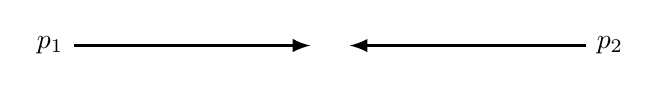
\begin{tikzpicture}
            \draw[very thick, -latex] (0,0) node [left] {$\fvec p_1$} -- (3,0);
            \draw[very thick, latex-] (3.5,0) -- (6.5,0) node [right] {$\fvec p_2$};
        \end{tikzpicture}
    \end{center}
    \begin{align}
        s \defi \lb \fvec p_1 + \fvec p_2\rb^2 = \lb \fvec p_1 + \fvec p_2 \rb^\mu \lb \fvec p_1 + \fvec p_2 \rb_\mu 
    \end{align}
    is Lorentz invariant since it is a scalar product. Hence it is the same in all reference frames.
\end{example}
\paragraph{Four vector derivatives}
\begin{align}
    \pa_\mu = \pdv{x^\mu} \ra \lb \pa_t, \vec \grad \rb
\end{align}
transforms like a covariant vector. Whereas
\begin{align}
    \pa^\mu = \pdv{x_\mu} \ra \qty(t, - \vec \grad)
\end{align}
transforms like a contravariant vector. The ''scalar product`` of these two is the d'Alembert operator
\begin{align}
    \Box \defi \pa_\mu\pa^\mu = \pa_t^2 - \Lap\,,
\end{align}
\begin{compactitem}
    \item[with] the Laplace operator $\Lap = \vec \grad^2$.
\end{compactitem}

\section{Elementary particles}
\paragraph{Fermions (spin $\nicefrac 12$)} Lepton sector:
\begin{align}
    \mqty(\upnu_\mr{e} \\\mr e^- ), \quad \mqty(\upnu_\upmu \\ \upmu^-),\quad \mqty(\upnu_\uptau \\ \uptau^-) \qquad \text{with charges } \mqty{Q = 0 \\ Q= -\mr e}
\end{align}
They come with a certain mass hierarchy $m_\mr{e} < m_\upmu < m_\uptau$ and the assumption in the standard model that $m_\upnu = 0$ regardless of the neutrino flavour. However we know $m_\upnu >0$ but very small.

Quark sector:
\begin{align}
    \mqty(u \\ d), \quad \mqty(c \\ s), \quad \mqty( t \\ b) \qquad \text{with charges } \mqty{Q = \frac 23 \mr e \\ Q = - \frac 13 \mr e}
\end{align}
Free particles are bounded states with $qq'q''$ as baryons and $q\bar q$ as mesons. Additionally, only colour-neutral particle states are observed.

Both sectors come with the respective 6 anti-particles.

\paragraph{Bosons (spin $1$)} exchange particles of interactions
\begin{compactitem}
    \item[$\upgamma$:] em. interaction, $m=0$, $Q=0$ couples to electric charge
    \item[$Z^0$:] weak interaction, $m = \SI{91}{\giga\eV}$, $Q=0$, couples to weak charge
    \item[$W^\pm$:] weak interaction, $m = \SI{80}{\giga\eV}$, $Q = \pm \mr e$, couples to weak charge
    \item[$g$:] strong interaction, $m=0$, $Q=0$\\
    8 gluons in total, carry colour charge\\
    couple to quarks and to one another (''self-coupling``)
\end{compactitem}

\paragraph{Scalar (spin $0$)}
\begin{compactitem}
    \item[$H^0$:] Higgs boson, brings mass to $Z^0$, $W^\pm$ (''spontaneous symmetry breaking``)\\
    $m = \SI{125}{\giga\eV}$
\end{compactitem}

\section{Feynman diagrams}
These give pictorial representations of particle reactions. Perturbative expansion of scattering ''in a potential`` into leading order and higher order terms, if necessary.
\begin{example}
    electromagnetic scattering (leading order)
    \begin{multicols}{2}
        \begin{center}
            \begin{tikzpicture}
                \begin{feynman}
                \vertex (a1);
                \vertex [below right = 2cm of a1] (b1);
                \vertex [above right = 2cm of b1] (a2);
                \vertex [below = 2cm of b1] (c1);
                \vertex [below left = 2cm of c1] (d1);
                \vertex [below right = 2cm of c1] (d2);
                \vertex [below left = 0.5cm of d1] (z1);
                \vertex [right = 1.6cm of z1] (z2);
                \vertex [below right = 0.5cm of d2] (z4);
                \vertex [left = 1.6cm of z4] (z3);
                \vertex [below = 2.2cm of c1] (y1) {particles};
                \diagram*{
                (a1) -- [fermion, edge label = $\mr e^-$, momentum' = $\fvec p_1$] (b1) -- [fermion, edge label = $\mr e^-$, momentum' = $\fvec p_1'$] (a2),
                (b1) -- [photon, edge label' = $\upgamma$, momentum = $\fvec q$] (c1),
                (d1) -- [fermion, edge label' = $\upmu^-$, momentum = $\fvec p_2$] (c1) -- [fermion, edge label' = $\upmu^-$, momentum = $\fvec p_2'$] (d2);
                };
                \draw[decoration={brace}, decorate] (z2.south) -- node[below] {incoming} (z1.south west);
                \draw[decoration={brace}, decorate] (z4.south east) -- node[below] {outgoing} (z3.south);
                \end{feynman}
            \end{tikzpicture}
        \end{center}
        \begin{compactitem}
            \item[with] $\fvec q$: 4-momentum transfer
        \end{compactitem}
        We will describe this in $\fvec q^2$ (which is Lorentz invariant)
        \begin{align}
            \fvec q^2 = \qty(\fvec p_1 - \fvec p_1')^2 \neq 0
        \end{align}
        The inequity to zero means that it is off mass-shell\\
        $\Ra$ virtual particle because it carries to much/less energy
    \end{multicols}
    
    Next question to ask is: What is the \tb{transition amplitude}?
    \begin{multicols}{2}
        \begin{center}
            \begin{tikzpicture}
                \begin{feynman}
                    \vertex (b1);
                    \vertex [above left  = 1cm of b1] (a1) {$\mr e^-$};
                    \vertex [above right = 1cm of b1] (a2) {$\mr e^-$};
                    \vertex [below = 1cm of b1] (c1);
                    \vertex [below left  = 1cm of c1] (d1) {$\upmu^-$};
                    \vertex [below right = 1cm of c1] (d2) {$\upmu^-$};
                    \diagram*{
                        (a1) -- [fermion] (b1) -- [fermion] (a2),
                        (b1) -- [scalar, momentum = {$\fvec q, M$}] (c1),
                        (d1) -- [fermion] (c1) -- [fermion] (d2);
                    };
                \end{feynman}
            \end{tikzpicture}
        \end{center}
    \begin{align}
        amplitude \propto g_1 \frac{1}{\fvec q^2 - M^2} g_2
    \end{align}
    \begin{compactitem}
        \item[with] $g_{1,2}$: coupling strength between fermion and exchange particle
        \item[] $\nicefrac{1}{\fvec q^2-M^2}$: boson propagator for exchange particle of mass $M$
    \end{compactitem}
    \end{multicols}
    Here the electromagnetic and the weak interaction contribute, i.e.
    \begin{align*}
        \feynmandiagram[vertical= b to d, baseline = -2cm]{
        a [particle = $\mr e^-$] -- [fermion] b -- [fermion] c [particle = $\mr e^-$],
        b -- [photon, edge label = $\upgamma$] d,
        e [particle = $\upmu^-$]-- [anti fermion] d -- [anti fermion] f [particle = $\upmu^-$],
        };
        + 
        \feynmandiagram[vertical= b to d, baseline = -2cm]{
        a [particle = $\mr e^-$] -- [fermion] b -- [fermion] c [particle = $\mr e^-$],
        b -- [scalar, edge label = $Z^0$] d,
        e [particle = $\upmu^-$]-- [anti fermion] d -- [anti fermion] f [particle = $\upmu^-$],
        };
        = e \frac{1}{\fvec q^2}e + g_1 \frac{1}{\fvec q^2 - M_Z^2} g_2
    \end{align*}
    Last question: What is the \tb{cross section}?\\
    It is proportional to the transition probability
    \begin{align}
        \sigma \propto W, \qquad W \propto \qty| amplitude_1 + amplitude_2 |^2 \propto \frac{\mr e^4}{\fvec q^4}
    \end{align}
    The factor $\nicefrac{1}{\fvec q^4}$ leads to a rapid decrease of the cross section as momentum transfer increases.
    \begin{center}
        \begin{tikzpicture}
            \draw[-latex] (-3.25,0) node [left] {$\fvec p_1$} -- (-.25,0);
            \draw[latex-] (.25,0) -- (3.25,0) node [right] {$\fvec p_2$};
            \draw[-latex] (0,0,0) -- (3,1.5,0);
            \coordinate (O) at (0,0,0);
            \tdplotsetcoord{P1}{3.5}{90}{30};
            \tdplotsetcoord{P2}{3.5}{90}{20};
            \tdplotsetcoord{P3}{3.5}{30}{30};
            \tdplotsetcoord{P4}{3.5}{0}{30};
            \draw[-latex] (P1) -- (P2);% -- (P3) -- (P4) -- (P1);
            \draw[dashed] (3.5,90,30) arc (30:20:3.5);
        \end{tikzpicture}
    \end{center}
\end{example}